\documentclass[../Document.tex]{subfiles}
\graphicspath{{\subfix{../images/}}}

\begin{document}


\Chapter{MODELING VALID MOLECULES USING \acrshort{cp}}
\label{chap:cp-validity}

In this chapter, we will put forward a way to model that can represent valid molecules using \cp.
As mentioned previously, we choose to use \smiles to encode our molecules. This is a simple and easy-to-read one-dimensional molecule representation which can easily be modelled by \cp.

We first describe the grammar that was required to describe the \smiles language. This is the key component that allows our model to generate molecules in the right encoding. We will then give a formal definition for our model before finally explaining our experiments and results.


\section{\smiles Grammar}
\label{sec:smiles-valid-grammar}
\smiles was developed for applications in organic chemistry, this can be seen in some of its rules. For example, the addition of tokens to describe aromatic rings is something that was added to simplify the notation, specifically due to the common occurrence of these rings. Another example is that simple atom tokens with no descriptor tokens have an implied complete valence shell (\ie the atom is in its stable state). \smiles requires an explicit indication when an atom does not respect its valence shell, whether it has more or less than the expected amount. This is why the grammar we chose to use, which is a variation of the one described by Kraev in his work~\cite{kraev2018grammars}, ensures that atom valences are respected.

The original work uses masks in addition to this grammar to completely avoid invalid outputs.
The first mask handles numerical assignment for cycles, guaranteeing that cycles are numbered correctly.
The second mask avoids making cycles that are too small (\ie cycles of 2 atoms) and cycles that are too long. They limit their cycle length to 8 based on what they observe in their database~\cite{kraev2018grammars}.

\commented{Include important rules here from grammar}
We address both of these issues by modifying the base grammar and adding new constraints as will be discussed later. The final grammar used for validity can be seen in Appendix~\ref{annex:grammar-validity}.

\subsubsection{Padding}
For the purpose of using this grammar in our \cp model, we add padding tokens that can complete the end of a molecule. 
This will allow our model to generate any molecule up to the size instead of giving it a fixed length, allowing for a more versatile model.
We chose ``\_'' as our padding token.

An easy way to make this change is to create a new starting token that can be developed into the old start token and any number of padding tokens (including none). This change was not influential on the performance of the algorithm and allows for more options during generation.


\subsubsection{Hydrogen tokens}
Some Hydrogen tokens can be included in the molecule. These can be followed by a number to indicate the number of Hydrogen atoms present. We change these tokens to directly include the number.
Instead of needing two tokens (``H'' and ``3'') we now use one token (``H3'') made up of two characters.

This avoids confusing Hydrogen count tokens for cycle tokens and improves our model's understanding of what it is generating.


\subsubsection{Cycle-length limit}
The final required modification we make to our grammar is to limit the cycle length.
We wish to ensure that cycle lengths remain in the desired range (between 3 and 8 inclusively).
In datasets of known drug-like molecules, long cycles are infrequent.
In the dataset MOSES~\cite{MOSES}, containing near two million molecules, no molecule features anything greater than a length-6 cycle. However, in another dataset containing near 250 thousand molecules, Zinc\_250k~\cite{Akhmetshin2021}, we can find up to length-8 cycles.
This seems to indicate that long cycles are either undesirable or lead to chemically unstable molecules (\ie molecules that we cannot synthesize).

We achieve this by limiting the number of tokens that a cycle production can be developed into. This information must be encoded in nonterminals where a larger cycle nonterminal can be rewritten as an atom and a smaller cycle nonterminal as seen in Table~\ref{tab:grammar-cycle-degradation}.

\begin{table}[ht]
    \centering
    \begin{tabular}{r | l c l}
        1 & valence\_2 & $\rightarrow$ & valence\_4\_num1 ``('' cycle1\_n\_bond ``)'' \\
        2 & cycle1\_n\_bond & $\rightarrow$ & cycle1\_7\_bond \\
        3 & cycle1\_7\_bond & $\rightarrow$ & cycle1\_6\_bond \\
        4 & cycle1\_6\_bond & $\rightarrow$ & cycle1\_5\_bond \\
        5 & cycle1\_5\_bond & $\rightarrow$ & cycle1\_4\_bond \\
        6 & cycle1\_4\_bond & $\rightarrow$ & cycle1\_3\_bond \\
        7 & cycle1\_3\_bond & $\rightarrow$ & cycle1\_2\_bond \\
        8 & cycle1\_7\_bond & $\rightarrow$ & valence\_2 cycle1\_6\_bond \\
        9 & cycle1\_6\_bond & $\rightarrow$ & valence\_2 cycle1\_5\_bond \\
        & & \ldots & \\
        10 & cycle1\_2\_bond & $\rightarrow$ & valence\_2 valence\_2\_num1 \\
    \end{tabular}
    \caption[Cycle degradation example from the grammar]{Cycle degradation example from the grammar.
    Rule 1 shows how a cycle is started, in this case it is started in a branch. The nonterminal outside the branch, ``valence\_4\_num1'', is a part of the cycle and must be taken into account for the length.
    Rule 2 was added to easily change the starting size of the cycle.
    Rules 3-7 allow for cycles to get smaller without adding another token, this is how we allow smaller cycles than 8.
    Rules 8-10 are the development of the cycle, we add a nonterminal and go down to the cycle size down.
    Rule 10 is special since it is the end of a cycle, so we first place a nonterminal followed by a nonterminal that is numbered to indicate the end of the cycle.
    The name of the cycle nonterminal contains information on what it will develop into: ``cycle1'' means it is the cycle identified by the ``1'' token, ``\_n\_'' indicates how many more atoms this nonterminal will develop into, ``bond'' tells us that it is a simple bond that is expected.}
    \label{tab:grammar-cycle-degradation}
\end{table}

This change alone guarantees that any nonterminal ``num'' will have another nonterminal ``num'' within an acceptable distance.
However, this does not guarantee that the nonterminal ``num'' will be developed into the same cycle number.
Take the unfinished chain ``C\textit{num}CCCCC\textit{num}NC\textit{num}CCCCC\textit{num}'' as an example.
While we would expect the finished chain to be ``C1CCCCC1NC2CCCCC2'', the current grammar would also accept \\
``C1CCCCC2NC2CCCCC1'', which results in both cycles being the wrong size.

This was a problem we ran into fairly quickly after applying the cycle size limit changes to the grammar, resulting in one very long cycle and one small one instead of two appropriate cycles. The solution was to integrate into the left-hand side of the production information about which cycle is being developed as can also be seen in Table~\ref{tab:grammar-cycle-degradation}.

As Kraev mentions in the original paper\cite{kraev2018grammars}, this change will make the grammar grow very quickly in size based on the maximum number of cycles allowed (not to be confused with the maximum cycle-length).
Therefore, it was critical to limit the number of cycles to avoid drastically increasing the size of our grammar.
After examining the two datasets at our disposal, 6 molecules from the ZINC250K dataset~\cite{Akhmetshin2021} and 4 from the MOSES~\cite{MOSES} dataset exceed 6 cycles. These datasets contain, respectively, 250K and 2M molecules. Based on this, we decided to limit the number of cycles to 6, seeing as it does not exclude many molecules from the ones observed in the known drugs datasets.

All of these changes ensure that cycles have an appropriate length. However, this does increase the size of the grammar. While the original \gls{cfg} from Kraev contained 34 terminals, 36 nonterminals and 138 productions, the current \gls{cfg} now has 32 terminals, 194 nonterminals and 538 productions.

We have two fewer terminals overall because we removed 3 cycle numbering tokens (``7'', ``8'', ``9'') as well as the token that is used to number cycles using two digits (``\%''). However, we did add the padding token, ``\_'', and we added the ``H3'' token to fully distinguish cycle numbering tokens from other numeric tokens. Notice we did not add the ``H2'' token as it was not present in the grammar previously.


\section{Our Model}
This section will first describe our model's variables and their domains.
We will then go over formal definitions of the constraints used to model valid molecules and break certain easily-identifiable symmetries.
Following the validity constraints, we define constraints that target specific structures in our generated molecules.
Finally, we will define the constraints required to target desirable properties.


\subsection{Variables}
We chose to limit the size of our molecules to 40 tokens. Since we use padding tokens, this means we can model any molecule of size 40 or less, which represents 83\% of all molecules in the two datasets we chose to use in our work (ZINC250K and MOSES).
This decision ensures the problem is representative of real-life molecules observed in our datasets and hence provides a meaningful empirical study.

We define 40 variables, one for each token in the molecule such as $\mathcal{X} = {X_1, X_2, \dots, X_{40}}$. Each token starts with the same domain, containing every possible terminal in the \smiles grammar alphabet.

This is formally defined as 
\begin{center}
$D(X_i) = $\{
    Br, Cl, F, I, C, N, O, S, c, n, o, s, 1, 2, 3, 4, 5, 6, (, ), =, \#, [, ], +, -, H, H3, /, \textbackslash, @, \_
\}
\end{center}

This setup allows any combination of \smiles tokens of size 40, including invalid ones. To ensure validity, we use three constraints as described in the following subsection.


\subsection{Validity Constraints}
\label{sec:validity-constraint-definition}
This section will answer our first research question: Can we use \acrshort{cp} to model valid molecules using a one-dimensional encoding?
With the following constraints, our model will be able to model valid \smiles molecules.

\subsubsection{Grammar Constraint}
The grammar constraint is responsible for guaranteeing the \smiles syntax in our generated molecules. The grammar constraint is a global constraint applied to all variables in the model. It also requires the \gls{cfg} that we defined earlier in Section~\ref{sec:smiles-valid-grammar}.

$$
    \texttt{grammar}(\langle X_1, X_2, \ldots, X_{40} \rangle, \mathcal{G}_{\texttt{SMILES}})\\
$$

This constraint does a lot of the work in ensuring that the generated output is a valid \smiles string. It guarantees:
\begin{enumerate}
    \item No valence mistakes. Atoms used in the molecule will respect the expected number of bonds to complete their valence shell.
    \item Opened cycles are appropriately paired to another cycle token to close it.
    \item Cycles respect a maximal length to avoid non-sensically large cycles that do not appear in drug-like molecules in known datasets.
    \item Any branch token has a corresponding opening/closing branch token.
\end{enumerate}

This constraint on its own would already generate valid \smiles strings. However, we add two more constraints to improve the readability of our generated results and avoid symmetries.

\subsubsection{Cycle Parity Constraint}
The cycle parity constraint ensures that all cycle tokens in the grammar's alphabet are used either twice or never. This avoids having two cycles with the same cycle identifier. In classic \smiles notation, the same cycle identifier can be reused if there is no ambiguity.

We decided not to allow the reuse of cycle tokens, since adding checks to avoid ambiguity in the grammar would make it much more complex, as we would need to track which cycles are currently open at all times. This simple constraint avoids the generation of ambiguous molecules while avoiding a larger grammar that would have taken a long time to design.

$$
    \among(\langle X_1, X_2, \ldots, X_{40} \rangle, \{j\}, \{0,2\})\ \forall\ j\ \vert\ 1 \leq j \leq 6
$$

\subsubsection{Cycle Numbering Constraint}
\label{sec:cycle-numbering-constraint}
The cycle numbering constraint is a symmetry-breaking constraint. It avoids using larger cycle identification tokens before smaller ones. In other words, the first opened cycle is identified using the token ``1'', the second will be identified using ``2'' and so on and so forth.
This ensures there is only one possible cycle token choice every time a cycle token is placed.

This constraint is considered to be symmetry-breaking since it avoids exploring branches where a ``1'' would be replaced by a ``2'' without any other changes.

We represent this using a \regular constraint which ensures the variables it is placed upon respect a given automaton. The automaton defined in Figure~\ref{fig:cycleCountingAutomaton} ensures that, at any given state, we can freely place any cycle token already encountered. It also guarantees that only the next smallest cycle token can be used, excluding the ones already encountered, and using it transitions us to the next state.

$$\regular(\langle X_1, X_2, \ldots, X_n \rangle, \mathcal{A})$$

\begin{figure}[ht]
    \centering
    \begin{tikzpicture}
        \tikzset{
            ->, % makes the edges directed
            node distance=2.5cm, % specifies the minimum distance between two nodes. Change if necessary.
            every state/.style={thick, fill=gray!10}, % sets the properties for each ’state’ node
            initial text=$ $, % sets the text that appears on the start arrow
        }
        \node[state, initial] (S) {start};
        \node[state, right of=S] (q1) {1 cycle};
        \node[state, right of=q1] (q2) {2 cycles};
        \node[right =0.5cm of q2] (skip_1) {$\cdots$};
        \node[state, right =0.5cm of skip_1] (qi) {i cycles};
        \node[right =0.75cm of qi] (skip_2) {$\cdots$};
        \node[state, right =0.5 of skip_2] (q6) {6 cycles};

        \draw
        (S) edge[loop above] node{$\Sigma \setminus \{1,\ldots,6\}$} (S)
        (S) edge[above] node{1} (q1)
        (q1) edge[loop below] node{$\Sigma \setminus \{2,\ldots,6\}$} (q1)
        (q1) edge[above] node{2} (q2)
        (q2) edge[loop above] node{$\Sigma \setminus \{3,\ldots,6\}$} (q2)
        (q2) edge[above] node{3} (skip_1)
        (skip_1) edge[above] node{i} (qi)
        (qi) edge[loop below] node{$\Sigma \setminus \{i+1,\ldots,6\}$} (qi)
        (qi) edge[above] node{i+1} (skip_2)
        (skip_2) edge[above] node{6} (q6)
        (q6) edge[loop above] node{$\Sigma$} (q6)
        ;
    \end{tikzpicture}
    \caption[Automaton $\mathcal{A}$ which imposes ordinal order on cycle numbering.]{Automaton $\mathcal{A}$ which imposes ordinal order on cycle numbering. The starting state has no cycles that have been opened yet and subsequent states each contain one more opened cycle than the last. The $\Sigma$ character represents all terminals in the grammar's alphabet. Every token, other than certain cycle tokens, lead back to the same state. Starting at the first state after the start state, cycle tokens that have already been seen can be placed freely.}
    \label{fig:cycleCountingAutomaton}
\end{figure}


\subsection{Structural Constraints}
\label{sec:structural-constraints-definition}
This section will present two constraints targeting specific structures in generated molecules. These constraints will be used to get samples of varying difficulty during our experiments. These constraints will never be used on their own, instead always being used in tandem with the validity constraints from Section~\ref{sec:validity-constraint-definition}.

\subsubsection{Cycle Count Constraint}
This constraint forces our generated output to contain a certain number of cycles. 
Using \smiles notation, this is very simple to do.
By previously placing the cycle numbering constraint, we guarantee that each cycle has its own number token used to identify it.
This allows us to use an \among constraint, requiring the presence of the number token equivalent to the number of desired cycles, \eg if we want 4 cycles, we require the presence of the token ``4''.

While this ensures we get 4 cycles, it actually ensures we get \textit{at least} 4 cycles. To avoid getting more than 4, we have to place a second \among constraint that forbids the use of the next smallest cycle token. In our example where we have 4 cycles, we would forbid the use of the token ``5''.

Formally this is defined using the two following constraints where $N_c$ is the number of desired cycles in the chain. It is important we ask for 2 and not 1, since the cycle parity constraint from Section~\ref{sec:validity-constraint-definition} already restricts the number of appearances to either 0 or 2. 

\begin{align*}
    &\among(\langle X_1, X_2, \ldots, X_{40} \rangle, \{N_c\}, 2)\\
    &\among(\langle X_1, X_2, \ldots, X_{40} \rangle, \{N_c+1\}, 0)
\end{align*}


\subsubsection{Branch Count Constraint}
Similarly to the previous constraint, the branch count constraint requires a certain number of branches in the generated output. Since the grammar constraint from Section~\ref{sec:validity-constraint-definition} ensures that any opened branch is closed, we can constrain the number of total branches by placing an \among constraint on either the opening or closing branch tokens. In the following definition, $N_b$ is the desired number of branches.

$$
    \among(\langle X_1, X_2, \ldots, X_{40} \rangle, \{``("\}, N_b)
$$


\subsection{Molecular Property Constraints}
\label{sec:property-constraints-definition}
In this section, we answer our second research question: Can we use \acrshort{cp} to model desirable molecular properties in \acrshort{smiles} molecules?

We previously talked about Lipinski's rule of five in Section~\ref{sec:lipinski-rules}. We will show how it is possible to describe each of these properties using constraints in our current model.

These constraints will never be used alone, they are always used with the constraints from Section~\ref{sec:validity-constraint-definition}.

Due to the two Hydrogen-bond constraints we will define later, the grammar we use has to be modified and, in its \gls{cfg} form, now has 35 terminals, 195 nonterminals and 607 productions.

\subsubsection{Molecular Weight Constraint}
The first property constraint is the molecular weight.
Since the solver we use only allows for integers, we multiply all weight values by 10 to get more precision for this constraint.

\paragraph{Estimating the weight of the grammar's tokens.}
Since we are working on a one-dimensional representation, \smiles, we attempt to estimate the weight of the total molecule by estimating the weight of each token in the \smiles string.
However, this isn't as simple as linking atoms to their atomic weight, since we have to account for the Hydrogen atoms that are potentially bonded but implicit in \smiles notation.

An intuitive solution to this is to assume that each atom token is making two bonds, one on its left and one on its right in the \smiles chain.
This allows us to assume that each atom token is bonded to two less Hydrogen atoms than the number of bonds needed to complete its valence shell, \eg Carbon, which needs to make 4 bonds to complete its valence shell, would have an assumed 2 bonds with Hydrogen atoms.

However, this sometimes results in an overestimation of the molecule's weight.
To correct this, we associate a weight, which is sometimes negative, to non-atomic tokens.

Cycle tokens are an extra bond that our current weight model does not account for.
Each extra bond is a bond that cannot be made with a Hydrogen atom.
For that reason, we associate all our cycle tokens to the negative weight of a Hydrogen atom.

It would seem like branch tokens need special weights for the same reason.
However, the opening branch token indicates an extra bond (\ie a negative weight) while the closing branch token indicates a lacking bond that we assumed was present (\ie a positive weight).
Overall, these two tokens should cancel out. However, this is only true if the token to the left of the closing branch token was expected to make a bond on its right. If the last atom already has a full valence shell, \eg ``\ldots F)'' or ``\ldots =O)'', it cannot bond with another on its right. In such cases, our assumption that the closing branch token ``replaced'' one of the atom's bonds is wrong and would result in a slightly higher weight than expected.

Bond tokens are also associated to negative weights.
When we make a double bond, there are two fewer Hydrogen atoms than we assumed there would be in our atom weights.
Similarly, a triple bond means there are four fewer Hydrogen atoms bonded to the two atoms around the bond token.
Therefore, the double and triple bond tokens are, respectively, associated to a weight of -20 and -40.

We also had to adjust the weight of aromatic cycle tokens.
As we explained earlier in Section~\ref{sec:molecule-encodings}, aromatic cycles are a specific type of cycle where single and double bonds alternate.
This is common enough to justify a shorthand notation in \smiles.
We can assume that these atoms are bonded to 3 other atoms, unlike the 2 bonds for non-aromatic atoms, \eg the aromatic variant of Carbon would have 1 Hydrogen atom bonded to it instead of 2 and its associated weight would reflect this.

\commented{Tu ne dis pas que tu as fait une régression linéaire. Ces poids sur les jetons ne sont quand même pas le "ground truth" mais une approximation statistique. Donc tu es quand même justifié d'avoir utilisé tes poids. Dis simplement que ces tests confirment que les poids que tu as dérivés manuellement donne une bonne approximation du poids réel.}

\gilles{Ces tests sont avant la r\'egression lin\'eaire, c'\'etait quand on regardait ce qui cause les erreurs et on a trouv\'e qu'en mettant un poids de 10 pour le ``+'', on obtient des meilleurs r\'esultats}

Finally, we did some testing to see the accuracy of our estimation.
We used the open-source tool RDKit\footnote{https://www.rdkit.org/} to calculate the true weight.
During our tests, we found that associating a positive weight to the ``+'' token improved the score.
Atoms with a charge have a different number of Hydrogen atoms bonded to them.

With this we create a weight array (Table~\ref{tab:token-weight-map}), ${\cal T}^w$,  indexed by token IDs.

\begin{table}[H]
    \centering
    \begin{tabular}{c|c|c}
        Token & Human Weight & Linear Regression Weight\\
        \hline
        C & 140 & 140\\
        c & 130 & 130\\
        N & 150 & 148\\
        n & 140 & 144\\
        O & 160 & 161\\
        o & 160 & 158\\
        S & 321 & 338\\
        s & 321 & 319\\
        F & 180 & 180\\
        Cl & 345 & 346\\
        Br & 789 & 793\\
        I & 1259 & 1259\\
        = & -20 & -13\\
        \# & -40 & -35\\
        + & 10 & 11\\
        - & 10 & -1\\
        1 & -10 & -9\\
        2 & -10 & -9\\
        3 & -10 & -9\\
        4 & -10 & -9\\
        5 & -10 & -9\\
        6 & -10 & -9\\
        $($ & 0 & 1\\
        $)$ & 0 & 1\\
        $[$ & 0 & -4\\
        $]$ & 0 & -4\\
        H & 0 & 12\\
        H2 & 0 & 18\\
        H3 & 0 & 19\\
        @ & 0 & -3\\
        / & 0 & -5\\
        \textbackslash & 0 & -9
    \end{tabular}
    \caption[Estimated token to weight array ${\cal T}^w$]{Estimated token to weight array ${\cal T}^w$. Any token that is not present in this weight map has a weight of 0. The middle column are the weights using our human intuition, the right column are the weights as predicted by the linear regression. While there are some differences, most weights are similar which confirms our intuition. However, we continue to use the human weights in our experiments.}
    \label{tab:token-weight-map}
\end{table}

\paragraph{Defining the constraint.}
To apply this constraint, we first create weight variables, $W_i$, that will represent the weight of their associated token variables, $X_i$.

We link the values of these variables using the \element constraint. It uses the weight array previously defined, ${\cal T}^w$ as a lookup table and ensures that $W_i$ is the value associated to index $X_i$.

Once these variables are defined, we can constrain the sum, $S^w$, of the variable array, $W$, to our desired estimated value. To respect Lipinski's rule of five, we would limit the value to 500 Daltons (in our model, we would instead use 5000 since we multiply values by 10 for more significant numbers).


\begin{align*}
    &\element({\cal T}^w, X_i, W_i)\ \forall\ i\ \vert\ 1 \leq i \leq n \\
    &\somme(\langle W_1, W_2,\ldots,W_n \rangle, S^w) & & \\
    &S^w \leq 500  & &
\end{align*}

\paragraph{How accurate is this estimation?}
As mentioned previously, we tested this process on the 2.2M molecules in the two datasets used thus far in our work. On average the error is $1.06\%$ of the molecule's real weight. However, at its maximum, we find errors of $4.83\%$.

We include a graph of the distribution of relative error frequencies in Figure~\ref{fig:initial-weight-estimation}. Since it is an estimation, the relative error rate is acceptable and doesn't stop us from targeting a desirable region of the search space.

\begin{figure}[ht]
    \centering
    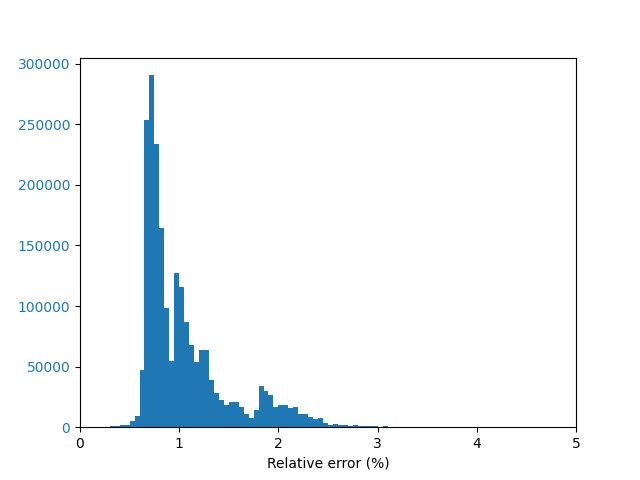
\includegraphics{weight_hist_real.png}
    \caption[Relative error frequency when estimating the weight of molecules using human intuition]{Relative error frequency when estimating the weight of molecules using human intuition. Most values are concentrated around 1\%, but we see nearly 50k molecules with errors around 2\%. We know the maximum error is 4.85\%, but it is so infrequent that it does not show up in the graph.}
    \label{fig:initial-weight-estimation}
\end{figure}

\paragraph{Can we improve this using a simple linear regression?}
By using a linear regression, we can see how close our intuition was and get a potential improvement to our current constraint.

We first convert all our molecules into frequency arrays, where each position contains the number of times the associated token shows up in the molecule. We can then use the python library \texttt{SKLearn} to do a linear regression and find weights for each token.

This leads to a good improvement on the average error, now of $0.23\%$, and a massive reduction in the maximum error, now of $2.80\%$. The results can be seen in Figure~\ref{fig:linreg-weight-estimation}.

While the linear regression's weights do vary from our own, they are mostly similar as can be seen in Table~\ref{tab:token-weight-map}. This confirms our intuition but goes to show that there is room for improvement.

\begin{figure}[ht]
    \centering
    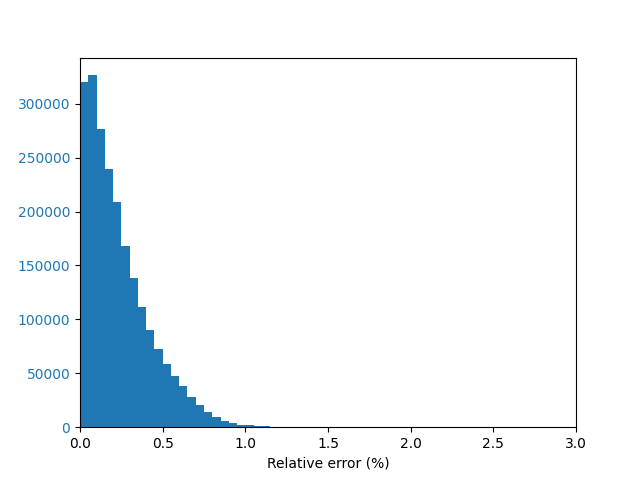
\includegraphics{weight_hist_lin_reg.png}
    \caption[Relative error frequency when estimating the weight of molecules using a linear regression]{Relative error frequency when estimating the weight of molecules using a linear regression.}
    \label{fig:linreg-weight-estimation}
\end{figure}


\subsubsection{Hydrogen-Bond Acceptors Constraint}
This property is simple enough to represent in \smiles notation. As long as one of the atoms of interest (\ie N, O, S) have a free electron pair, they are considered an acceptor. For these atoms to not have a free electron pair would require it to be used to make another bond and for its valence shell to be overloaded (\ie making more bonds than what is expected). This is possible but not common, and so a good estimation of the number of Hydrogen-bond acceptors in a molecule is simply the number of relevant atoms, \ie Nitrogen, Oxygen and Sulfur.
The aromatic version of the atoms are included in the constraint.

While Fluorine is an electronegative, Lipinski's rule of five specifically excludes it from the list of potential Hydrogen-bond acceptors\cite{LIPINSKI20013}.

We note the number of wanted acceptors as $N_a$ in the formal definition below.

\begin{align*}
    &\among(\langle X_1, X_2, \ldots, X_n \rangle, \{``N",``O",``S",``n",``o",``s"\}, N_a)\\
    &N_a \leq 10
\end{align*}


\subsubsection{Hydrogen-Bond Donors Constraint}
This property, while similar to the previous one, requires changes to our grammar in order to be represented correctly. The full changes can be seen in Appendix~\ref{annex:grammar-lipinski}.

Since our grammar already accounts for the number of bonds that atoms are making, it seemed natural to change certain productions to determine which atoms were donors and which ones weren't. However, this implies the need for new atom tokens to differentiate between the donor and non-donor version of the same atom. We add:
\begin{itemize}
    \item ``$N_D$'' as the donor version of ``N''
    \item ``$O_D$'' as the donor version of ``O''
    \item ``$S_D$'' as the donor version of ``S''
\end{itemize}

Since the atoms in question have to be bonded to a Hydrogen atom to be Hydrogen-bond donors, we suppose that they cannot be donors if they are a part of an aromatic cycle. For that reason, only the non-aromatic version of the atoms are included in the constraint.

Once we have modified our grammar, it is simply a matter of limiting how many of the donor tokens appear in our molecule. We note the number of wanted donors as $N_d$ as seen below.

\begin{align*}
    &\among(\langle X_1, X_2, \ldots, X_n \rangle, \{``T",``X",``R"\}, N_d)\\
    &N_d \leq 5
\end{align*}


\subsubsection{LogP Constraint}
To model the \emph{logP} value using only \smiles notation, another of Lipinski's rules, human ingenuity is not enough.

\paragraph{Ridge Regression.}
Basing ourselves on the work done previously by Vidal et al.~\cite{lingos}, we use a linear regression to estimate the partial contribution, positive or negative, of sequences of four tokens (\emph{$4$-grams}) on the \emph{logP} score.
In their work, they used a partial least squares regression to estimate the \emph{logP} value of different molecules.
Their results indicate that their model could accurately predict \emph{logP} values.
Similarly, we compute the partial contribution of every possible $4$-gram in the datasets by using a ridge regression (a linear regression where we add a small value to the input to avoid linearly dependant inputs).

The accuracy of this model is very variable. We did a relative error analysis as well as an absolute error analysis as can be seen in Table~\ref{tab:lingo-error-analysis}.

\paragraph{Absolute Error Analysis.} The first thing to note is that the average error sits at $0.1235$, an acceptable value when we are targeting a \emph{logP} score under $5$. However, the maximum error is much bigger, at $2.2231$. To get a clearer message, we calculate the median error (\ie the second quartile) and find that it is lower than our average, at $0.0861$. We decide to exclude outliers in our data by using the IQR filtering method. This filters out $4.56\%$ of our data as outliers and gives us our new average: $0.1063$.

\paragraph{Relative Error Analysis.} Relative error allows us to get a better picture by comparing the error to the targeted value instead of keeping an absolute scale. 
With an average error of $12.56\%$, our method doesn't seem too accurate.
However, our maximum error of $108'851.38\%$ seems absurd.
Upon further inspection, we found that we were getting these absurdly high relative errors on molecules with very small \emph{logP} scores (\ie smaller than $0.001$).
Since the relative error has the true value as the denominator, this makes the relative error for this sample grow disproportionately.
Once again, we looked at the median value, which is less sensitive to outliers and find that it is four times smaller than our current average at $3.68\%$.
To avoid falsifying our average with outliers, we filter our data using IQR filtering, filtering out $7.86\%$ of our data.
This allows us to get a more reliable average of $4.54\%$ relative error, a very acceptable error rate for our estimations.

\begin{table}[H]
    \centering
    \begin{tabular}{|c|c|c|}
        \hline
        Calculated Value & Absolute & Relative\\
        \hline
        Total Average Error & $0.1235$ & $12.56\%$\\
        \hline
        Total Maximum Error & $2.2231$ & $108'851.38\%$\\
        \hline
        Q1 & $0.0388$ & $1.56\%$\\
        \hline
        Q2 & $0.0861$ & $3.68\%$\\
        \hline
        Q3 & $0.1715$ & $8.02\%$\\
        \hline
        Inlier Data Coverage & $95.44\%$ & $92.14\%$\\
        \hline
        Inlier Average Error & $0.1063$ & $4.54\%$\\
        \hline
    \end{tabular}
    \caption[Error analysis on the \emph{logP} estimation constraint]{Error analysis on the \emph{logP} estimation constraint. The first two rows are the average and maximum error on all data points. The next three rows are the quartile values. We include a row to detail what percentage of the data points are still included after excluding outliers. The final row is the new average, excluding outliers, this gives us a better representation of our method's efficiency.}
    \label{tab:lingo-error-analysis}
\end{table}

\paragraph{Table Implementation.}
We can then create a table ${\cal T}^p$ which links every possible $4$-gram to its estimated contribution.
In the case where a $4$-gram has no or a very small partial contribution, its weight is set to 0, thus having no effect on the final estimation of the \emph{logP} value.

Our model then uses a \extensional constraint as defined below:

\begin{align*}
    &\extensional(\langle X_i,\ldots,X_{i+3},P_i\rangle, {\cal T}^p)\ \forall\ i\ \vert\ 1 \leq i \leq n-3 \\
    &\somme(\langle P_1, P_2,\ldots,P_{n-3} \rangle, S^p)\\
    &S^p \leq 5
\end{align*}

However, this table can potentially be quite large (the number of terminal tokens elevated to the power 4), we limit its size through the use of a wildcard token ($\star$) and the \shortTable constraint~\cite{DBLP:conf/aaai/VerhaegheLS17}.

\paragraph{Short Table Implementation.}
Since a $\star$ token can represent any other token, we can use it to map large numbers of zero-weight $4$-grams to the appropriate weight.
To identify the $4$-grams to which we can apply these wildcards, we iterate on each position and on all possible tokens for that position, if no important $4$-grams (that have a non-zero weight) contain the prefix, we associate that prefix followed by wildcard tokens to a weight of 0.
This wildcard allows us to reduce the table down to 39305 $4$-grams that have a non-zero weight, which is 3\% of all the possible $4$-grams. The total table, including zero weight $4$-grams, has $168'731$ rows, closer to $12.6\%$ of the size a normal \extensional constraint would have needed.

The constraint definition doesn't change much, we replace the \extensional constraint by a\\ \shortTable constraint and use the new table, ${\cal T}^{p\star}$:

\begin{align*}
    &\shortTable(\langle X_i,\ldots,X_{i+3},P_i\rangle, {\cal T}^{p\star})\ \forall\ i\ \vert\ 1 \leq i \leq n-3 \\
    &\somme(\langle P_1, P_2,\ldots,P_{n-3} \rangle, S^p)\\
    &S^p \leq 5
\end{align*}

This representation results in a number of constraints which grows linearly with the number of token variables. However, there is a way to represent this property by using a single \costregular constraint applied on the entire variable array $X$.

% ShortCT Yes BP:
% Constrain: 2.000 s
% Made DFS : 8.182 s
% exec time: 1.260 s
% Bad molecules (too short, no random it seems)

% ShortCT No BP:
% Constrain: 01.968 s
% Made DFS : 15.650 s
% exec time: 22.226 s
% Good molecules

% Regular:
% Constrain: 02.844 s
% Made DFS : 30.499 s
% exec time: 20.472 s



\paragraph{Cost Regular Implementation}
To implement this constraint using a \costregular, we have to remap our ${\cal T}^{p\star}$ table into an automaton $\mathcal{A}^p$.

This automaton contains a state for each non-zero weight $4$-gram as well as states for every $3$-gram, $2$-gram and $1$-gram necessary to get to the non-zero weight $4$-grams.
The transition to a $4$-gram state is associated to the partial contribution of that $4$-gram.
All other state transitions have a weight of 0 and all states in the automaton are considered valid final states.
See Algorithm~\ref{algo:logp-regular} to see exactly how we create the transition and weight table for our automaton.

The final automaton has $41'741$ states, a considerable reduction in size compared to the previous \shortTable constraint.

\begin{align*}
    &\costregular(\langle X_1, X_2, \ldots, X_n \rangle, \mathcal{A}^p, {\cal W}_{\mathcal{A}^p}).
\end{align*}

\begin{figure}[ht]
    \centering
    \begin{tikzpicture}
        \tikzset{
            ->, % makes the edges directed
            node distance=2.5cm, % specifies the minimum distance between two nodes. Change if necessary.
            every state/.style={thick, fill=gray!10}, % sets the properties for each ’state’ node
            initial text=$ $, % sets the text that appears on the start arrow
        }
        \node[state, initial] (S) {start};
        \node[state, right of=S] (s1) {a};
        \node[state, right of=s1] (s2) {ab};
        \node[state, right of=s2] (s3) {abb};
        \node[state, right of=s3] (s4) {abba};

        \draw
            (S) edge[loop above] node{$\Sigma$:0} (S)
            (S) edge[bend left=20, above] node{a:0} (s1)

            (s1) edge[loop above] node{a:0} (s1)
            (s1) edge[bend left=20, above] node{b:0} (s2)
            (s1) edge[bend left=20, above] node{$\Sigma$:0} (S)

            (s2) edge[bend left=20, above] node{a:0} (s1)
            (s2) edge[above] node{b:0} (s3)
            (s2) edge[bend left=40, above] node{$\Sigma$:0} (S)

            (s3) edge[above] node{a:\textcolor{red}{2.4}} (s4)
            (s3) edge[bend left=50, above] node{$\Sigma$:0} (S)
            
            (s4) edge[bend right=50, above] node{a:0} (s1)
            (s4) edge[bend right=40, above] node{b:0} (s2)
            (s4) edge[bend left=60, above] node{$\Sigma$:0} (S)
        ;
    \end{tikzpicture}
    \caption[Simplified example of automaton $\mathcal{A}^p$, associating a weight to a sequence during generation.]{Simplified example of automaton $\mathcal{A}^p$, associating a weight to a sequence during generation. This example associates a weight of $2.4$ to the $4$-gram \textbf{\texttt{abba}}. For clarity and simplicity, we limit ourselves to one sequence as the graph quickly becomes very connected. The only transition that has an associated weight is the one that completes the $4$-gram. Each state has a transition back to the start state in the case where it receives a token that is in the alphabet ($\Sigma$) but does not have its own state. For all transitions that have $\Sigma$ associated to them, we assume any tokens that are in another transition are excluded from $\Sigma$.}
    \label{fig:costregular-constraint-automaton}
\end{figure}

\begin{algorithm}[]
    \caption{\textbf{regularAutomatonCreation}$(N,w,g)$}
    \label{algo:logp-regular}
    \KwIn{\\
        \quad A list of non-zero weight $4$-grams: $N$;\\
        \quad A dictionary mapping each $4$-gram to its weight: $w$;\\
        \quad A list of the tokens in the grammar's alphabet: $g$
    }
    \KwOut{\\
        \quad A transition matrix: ${\cal T}_{A^p}$;\\
        \quad A weight matrix: ${\cal W}_{A^p}$;\\
    }

    \tcp{Define a state set that starts with the empty state}
    $\mathsf{S} \gets \{ ``" \}$\;

    \tcp{Find all relevant states from our $4$-grams}
    \ForEach{$\mathsf{ngram} \; \in N$} {
        $\mathsf{state} \gets ``"$\;
        \tcp{Add each partial sequence of the $4$-gram to the state set}
        \ForEach{$\mathsf{token} \; \in \mathsf{ngram}$} {
            $\mathsf{state} \gets \mathsf{state} + \mathsf{token}$\;
            $\mathsf{S} \gets \mathsf{S} \cup \mathsf{state}$\;
        }
    }

    \tcp{Fill the transition and weight matrix}
    \ForEach{$\mathsf{state} \; \in \mathsf{S}$} {
        \ForEach{$\mathsf{token} \; \in g$} {
            \tcp{Define the next state as the current state's last three tokens plus the given token}
            $\mathsf{state'} \gets \mathsf{state}[1:] + \mathsf{token}$\;
            \tcp{Remove the first token from the next state until we find a valid transition state. This will always default to the start state $``"$ if nothing is found.}
            \While{$\mathsf{state'} \notin \mathsf{S}$} {
                $\mathsf{state'} \gets \mathsf{state'}[1:]$\;
            }
            ${\cal T}_{A^p}[\mathsf{state}][\mathsf{token}] \gets \mathsf{state'}$\;
            \If{$\mathsf{\textbf{len}}(\mathsf{state'}) = 4$} {
                ${\cal W}_{A^p}[\mathsf{state}][\mathsf{t}] \gets w[\mathsf{state}]$\;
            }
        }
    }
    \Return (${\cal T}_{A^p}$, ${\cal W}_{A^p}$)\;
\end{algorithm}


\section{Experiments}
\label{sec:valid-experiments}
In the previous section, we've answered our first two research questions:

\begin{enumerate}
    \item Can we use \cp to model valid molecules in a one-dimensional encoding?
    \item Can we use \cp to model desirable molecular properties in \smiles molecules?
\end{enumerate}

In this section, our experiments will serve to answer the third of our questions: Can \bp be used to better guide a solver towards a solution?
These experiments will also serve to see the usefulness of the newly implemented weighted counting algorithm that was designed for the \grammar constraint.
The algorithm itself is out of scope for this paper, however these experiments were designed with the algorithm in mind.

There are two series of experiments: experiments on structural constraints and experiments on Lipinski's rule of five.

\subsection{Structural Experiments}
These experiments were run on an AMD Rome 7532 processor (2.4GHz, 256M cache L3) with 1 GB of \gls{ram} and using a 30-minute timeout. The results can be seen in Table~\ref{tab:structural-results}.

For these tests, we first apply constraints necessary for validity, then apply structural constraints and finally apply the molecular weight constraint.

\paragraph{Validity Constraints.} These will always be active in our tests as they are required to ensure the generated sequence respects \smiles.

\paragraph{Structural Constraints.} These constraints are used to diversify our experiments and run different instances of varying difficulty. This should give us a better overview of how different heuristics behave depending on the problem's complexity. We consider on every combination of number of cycles and branches in the respective ranges of 1\ldots3 and 2\ldots4. We note instance $\mathtt{c}i\mathtt{b}j$ as the instance corresponding to $i$ cycles and $j$ branches (in which case we add $N_b$ to $j$ and $N_c$ to $i$ in the corresponding pair of \among\ constraints seen earlier in Section~\ref{sec:structural-constraints-definition}).

\paragraph{Molecular Weight Constraint.} Long term structure increases a problem's complexity by making early decisions potentially have a significant impact on the generated sequence later. We target molecules close to the upper limit recommended by Lipinski's rule of five (\ie we constrain $S^w$ between 475 and 500 Daltons).

\subsection{Molecular Properties Experiments}
These experiments were run on an AMD Rome 7532 processor (2.4GHz, 256M cache L3) with 4 GB of \gls{ram} and using a 30-minute timeout. The results can be seen in Table~\ref{tab:property-results}.

We apply the validity constraints similarly to the previous experiments, however the structural constraints are not needed to generate more instances. This can be done directly with the rest of the molecular property constraints. All property constraints are applied to the model.

The validity constraints are identical to the ones in the previous experiments, there is nothing to add.

\paragraph{Molecular Weight Constraint.} This time, we vary the target range for the molecular weight constraint to generate instances of varying complexity. The ranges we use are: [175\ldots225], [275\ldots325], [375\ldots425]. These ranges give us an idea of the behavior while generating light, medium and heavy molecules. 

\paragraph{\emph{LogP} Constraint.} By varying the targeted \emph{logP} score, we get nine different instances similarly to the previous experiments. We choose the ranges: [-4,-3], [-2,-1], [1,2]. Note, none of our ranges include 0 as it may encourage the model to only use zero-weight $4$-grams. This behavior would be of little interest to us as we wish to show the advantages of \bp and this could be equivalent to disabling the constraint.

\subsection{Chomsky Normal Form}
All of our experiments require the \grammar constraint and since the solver we use, miniCPBP\footnote{\url{https://github.com/PesantGilles/MiniCPBP}}, requires a grammar in \gls{cnf} for its implementation, we develop a method to automate the transformation from the readable \gls{cfg} form to the desired \gls{cnf}. This allows us to keep working on the more readable \gls{cfg} format.

\gilles{Do I insert here from the intro? Or leave it where it is}

After converting the original grammar, the number of nonterminals and productions, respectively, increase to 169 and 411.
Meanwhile, the final grammar for the structural experiments grows to 640 nonterminals and 1996 productions. 
The grammar for the molecular property experiments is slightly larger in \gls{cfg} form, however, once converted to \gls{cnf} it remains comparable to the previous one with 642 nonterminals and 1990 productions. 
The difference between the two grammars should not be a significant factor in terms of time since they are of comparable size in every metric.

The complexity of the base propagation algorithm is cubic in regards to the number of variables as well as linear according to the number of productions~\cite{quimper2006}. The number of variables in our model does not change with the size of the grammar, however we do have nearly five times as many productions.
However, seeing as we are using Belief Augmented Constraint Programming, this requires an additional step which is also cubic in relation to the number of variables, linear in relation to the number of productions and linear in relation to the number of nonterminals.
So while the two modified grammars are of comparable size, they should both slow down the solver.

\subsection{Used Heuristics}
In our experiments, we include tests on three different heuristics.

\paragraph{domWDeg.} Being a learning-based heuristic, \texttt{domWDeg}~\cite{domwdeg} is run with restarts (initially after 100 fails and increased by a 1.5 factor), which is a common practice.
Early experiments on our instances confirmed that it generally performs better with restarts than without.
Its default value-selection heuristic, selecting the smallest value in the domain, performed very poorly, only managing to solve the first instance within our time limit.
Instead, we select a domain value uniformly at random and report the median of 11 runs. We consider an instance to have timed out if more than half the instances do so.

\paragraph{maxMarginalStrength.} \texttt{maxMarginalStrength}~\cite{GP:BP} is a branching heuristic based on the marginals computed by MiniCPBP using the weighted counting algorithm of each constraint in the model.
Because it is not learning-based and is deterministic, using restarts would not help.
We report on its use with standard depth-first search (\gls{dfs}) and also with \gls{lds} (\gls{lds}, with a maximum number of discrepancies starting at 1 and doubled at each iteration, ultimately making the search complete), which is a sensible option for a trusted branching heuristic~\cite{DBLP:conf/ijcai/HarveyG95}.


\section{Results}
This section will briefly go over our results as well as preliminary tests performed to determine which constraint \emph{logP} constraint to use.

\subsection{\emph{LogP} Comparison}
To determine which version of the \emph{logP} constraint to use, we ran a few preliminary tests and noted the time taken for each part of the process as well as the failures while exploring the search tree. The results can be seen in Table~\ref{tab:logp-constraint-time-analysis}.

\begin{table}[H]
    \centering
    \begin{tabular}{|c|c|c|c|}
        \cline{2-4}
        \multicolumn{1}{c|}{} & \textbf{Initial Setup (s)} & \textbf{Solve Time (s)} & \text{Failures}\\
        \hline
        \shortTable with \bp & $10.707$ & $1.168$ & $13$\\
        \hline
        \shortTable without \bp & $17.670$ & $24.116$ & $111$\\
        \hline
        \regular & $31.917$ & $20.944$ & $4$ \\
        \hline
    \end{tabular}
    \caption[Performance comparison between different implementations of the \emph{logP} estimation constraint]{Performance comparison between different implementations of the \emph{logP} estimation constraint. The addition of \bp clearly reduces the number of failures before a solution is found.}
    \label{tab:logp-constraint-time-analysis}
\end{table}

We initially compared the \shortTable and \regular constraints with \bp active for both. However, during our tests, we noticed that the \bp component of the \shortTable constraint would result in strange molecules. They were much shorter than previous tests (as small as the model could make them while still respecting all constraints) and had very little variety. We add the \shortTable constraint without \bp to our tests since, by disabling the \bp component, we find varied results of standard length again.

When looking at the results in Table~\ref{tab:logp-constraint-time-analysis}, \shortTable with \bp performs best in time.
However, we believe this is low solve time is due to the extremely short molecules it is generating. It would place at most 10 non-padding tokens before filling the rest of the sequence with padding.
Furthermore, it has to backtrack 13 times to find a small solution.
Meanwhile, the \regular constraint takes more time, but generates full length molecules with very few failures.
The \shortTable without \bp is dominated in every aspect by the other two candidates.
We settle on using the \regular constraint, preferring its low failure count and reliable results over the \shortTable equivalent.


\subsection{Structural Experiments}
The results to our structural experiments can be seen in Table~\ref{tab:structural-results}.

The \texttt{domWDeg/random} heuristic manages to solve all instances, however it can require in the thousands of fails.
Branching heuristics based on marginals make an integrated choice of variable and value.
The very low number of fails for \texttt{maxMarginalStrength} (several instances are even solved backtrack-free) is remarkable and shows the usefulness of the weighted counting algorithm for the \grammar constraint and of \bp as a whole.
There are four instances that are unsolved within the time limit, this is likely due to a bad decision early on in the search tree (as we are using a \gls{dfs}).
As can be seen by the results using \gls{lds}, all but one instance become solved, confirming our previous suspicion.
Even though, our \bp heuristics take more time per fail than their pure \cp counterpart, by quickly guiding the search towards a valid solution, \bp heuristics end up solving the problem faster in most cases.

\subsection{Molecular Properties Experiments}
The results to our structural experiments can be seen in Table~\ref{tab:property-results}.

Similarly to the previous experiments, the \texttt{domWDeg/random} heuristic performs well on most instances, leaving only one unsolved in the allocated time.
The advantage \bp gives to a solver can be seen much more clearly in these instances.
Almost every instance is solved with fewer than 10 backtracks when using \texttt{maxMarginalStrength}.
Unfortunately, the whether we use \gls{dfs} or \gls{lds} makes very little difference, and we cannot reliably say one method is better than the other in this instance.
However, while \texttt{maxMarginalStrength} does solve the problem with very few fails, the time to solve the instance is sometimes comparable to the pure \cp alternative.

Overall, these results once again confirm that constrained molecule generation is achievable using a \cp model such as the one described prior.
Although using the \grammar constraint is convenient, the aforementioned computational cost can be felt due to its large size.
It takes one second to post the constraint (including the initial propagation).
Running several iterations of \bp (including the weighted counting algorithm for \grammar) before branching takes three to four times longer than a branching heuristic such as \texttt{domWDeg}.
However, these are clearly offset by the superior search guidance, and thus, much smaller search tree.


\begin{table}[H]
    \centering
    \begin{tabular}{crrrrrr}
        \hline
        & \multicolumn{2}{c}{\texttt{domWdeg/random}} &  \multicolumn{2}{c}{\texttt{maxMarginalStrength/DFS}} & \multicolumn{2}{c}{\texttt{maxMarginalStrength/LDS}}\\
        instance & time(s) & fails & time(s) & fails & time(s) & fails \\
        \hline
        $\mathtt{c}1\mathtt{b}2$ & 20.2 & 103 &  8.9 & 0 & 8.9 & 0\\
        $\mathtt{c}1\mathtt{b}3$ & 14.0 & 65 &  12.0 & 0 & 11.7 & 0\\
        $\mathtt{c}1\mathtt{b}4$ & 61.7 & 484 & 12.2 & 0 & 12.6 & 0\\
        $\mathtt{c}2\mathtt{b}2$ & 26.3 & 105 &  -- & -- & 16.7 & 3\\
        $\mathtt{c}2\mathtt{b}3$ & 37.4 & 253 & 16.0 & 0 & 16.0 & 0\\
        $\mathtt{c}2\mathtt{b}4$ & 245.3 & 2083 &  17.9 & 12 & 17.5 & 6\\
        $\mathtt{c}3\mathtt{b}2$ & 131.2 & 1389 & -- & -- & 32.0 & 14\\
        $\mathtt{c}3\mathtt{b}3$ & 40.2 & 106 &  -- & -- & -- & --\\
        $\mathtt{c}3\mathtt{b}4$ & 101.5 & 1040 &  -- & -- & 498.8 & 247\\
        \hline
    \end{tabular}
    \caption[Comparing branching heuristics on some structurally-constrained molecule generation instances.]{Comparing branching heuristics on some structurally-constrained molecule generation instances. Instances marked with a blank line indicate a timed out instance. The number of fails indicates how many dead ends the solver ran into and had to backtrack to get out of. Since \texttt{domWdeg/random} incorporates randomness, we run 11 instances and report the median.}
    \label{tab:structural-results}
\end{table}


\begin{table}[]
    \centering
    \begin{tabular}{lrrrrrr}
        \hline
        & \multicolumn{2}{c}{\texttt{domWdeg/random}} & \multicolumn{2}{c}{\texttt{maxMarginalStrength/DFS}} & \multicolumn{2}{c}{\texttt{maxMarginalStrength/LDS}}\\
        instance & time(s) & fails & time(s) & fails & time(s) & fails \\
        \hline
        [175,225] [-4,-3]  & 287.6 &  66 & 200.3 & 30 & 173.4 & 2\cr
        [175,225] [-2,-1]  & 368.7 &  33 & 166.1 &  0 & 186.0 & 0\cr
        [175,225] [1,2]    &    -- &  -- & 190.5 &  6 & 233.6 & 9\cr
        [275,325] [-4,-3]  & 588.9 & 105 & 260.0 &  0 & 287.1 & 0\cr
        [275,325] [-2,-1]  & 217.2 &   5 & 287.2 &  0 & 279.8 & 0\cr 
        [275,325] [1,2]    & 209.7 &   5 & 282.6 &  0 & 321.3 & 0\cr 
        [375,425] [-4,-3]  & 527.8 & 231 & 160.7 &  2 & 179.2 & 1\cr 
        [375,425] [-2,-1]  & 401.4 & 121 & 140.6 &  1 & 160.4 & 1\cr 
        [375,425] [1,2]    & 199.8 &  23 & 187.0 &  0 & 141.4 & 0\cr 
        \hline
    \end{tabular}
    \caption[Comparing branching heuristics on some Lipinski-constrained molecule generation instances.]{Comparing branching heuristics on some Lipinski-constrained molecule generation instances. Instances marked with a blank line indicate a timed out instance. The number of fails indicates how many dead ends the solver ran into and had to backtrack to get out of. Since \texttt{domWdeg/random} incorporates randomness, we run 11 instances and report the median.}
    \label{tab:property-results}
\end{table}

\end{document}